\documentclass[11pt]{article}

% Change "review" to "final" to generate the final (camera-ready) version.
% Change to "preprint" to generate a non-anonymous version with page numbers.
\usepackage[review]{acl}

% Standard package includes
\usepackage{times}
\usepackage{latexsym}
\usepackage[T1]{fontenc}
\usepackage[utf8]{inputenc}
\usepackage{microtype}
\usepackage{inconsolata}
\usepackage{graphicx}

% Project additions
\usepackage{amsmath}
\usepackage{amssymb}
\usepackage{booktabs}
\usepackage{xcolor}

% Float placement: pack the appendix figure pages densely instead of leaving
% one figure per page. Affects layout only, never content.
\setcounter{topnumber}{3}
\setcounter{dbltopnumber}{3}
\setcounter{totalnumber}{5}
\renewcommand{\topfraction}{0.95}
\renewcommand{\dbltopfraction}{0.95}
\renewcommand{\bottomfraction}{0.90}
\renewcommand{\textfraction}{0.05}
\renewcommand{\floatpagefraction}{0.85}
\renewcommand{\dblfloatpagefraction}{0.85}

% ---------------------------------------------------------------------------
% Draft helpers. \pending{} marks numbers/claims NOT yet frozen (baselines,
% held-out confirmation, un-reproduced cells). They are meant to be greppable:
%     grep -rn "pending" paper/sections
% Remove the definition's colour for camera-ready, or redefine to \relax.
% ---------------------------------------------------------------------------
\newcommand{\pending}[1]{\textcolor{red}{[\textsc{pending}: #1]}}
\newcommand{\tbd}{\textcolor{red}{\scriptsize\textsc{tbd}}} % compact table placeholder
\newcommand{\frozen}[1]{#1} % semantic marker for verified numbers (no-op)

% Shorthands
\newcommand{\dsseven}{DeepSeek-R1-Distill-Qwen-7B}
\newcommand{\qweneight}{Qwen3-8B}
\newcommand{\pp}{\,\text{pp}}
\newcommand{\simplek}{simple@32}

\title{Stable Answers, Unfinished Reasoning: Why Self-Consensus\\ Is Not a Safe Early-Exit Signal}

% Anonymous for review.
\author{Anonymous ACL submission}

\begin{document}
\maketitle

\begin{abstract}
Reasoning language models produce long chains of thought, making
\emph{early exit}---stopping generation once the answer is settled---an
attractive way to cut inference cost. A popular family of methods
(e.g., Dynasor / Certaindex) periodically probes the partial trajectory for
its current answer and stops once probes \emph{agree}, betting that
intermediate consensus signals termination. We show this bet is unsafe, and
that the failure is not repaired by tuning the stopping rule within this family.
First, on \textsc{MATH}500 we document \emph{false consensus}: even a unanimous
window of recent probes is correct only $93.5\%$ of the time, and a naive
consensus stop loses $16.4$ percentage points (pp) of accuracy
($85.6\%\!\rightarrow\!69.2\%$) because continued reasoning frequently
overturns the intermediate answer. Second, we run a \emph{preregistered} search
over a seven-dimensional rule schema ($17{,}712$ candidate rules) on frozen
reasoning trajectories from two models and three math benchmarks, with
problem-grouped train/dev/test splits and stopping gates fixed in advance. On
the development set (held-out confirmation pending), \emph{no rule clears the
preregistered safety bar}: the safest stop still costs $1.85\pp$ per model.
Separately, under our dense-probe accounting, any rule with positive \emph{net}
token savings costs at least $4.87\pp$, and---counterintuitively---adaptive,
event-triggered probing is dominated by simple window consensus. We decompose
the cost into an intrinsic \emph{accuracy tax} (independent of probing) and a
\emph{probe tax} (a function of probe density), and argue only the accuracy tax
is probe-invariant. Our results suggest that safe early exit for reasoning
models likely requires a different termination signal, not a better-tuned
confidence threshold on probe agreement.
\end{abstract}

\section{Introduction}
\label{sec:intro}

Reasoning language models such as \dsseven{} and \qweneight{}
\citep{deepseekr1,qwen3,openai_o1} solve hard problems by emitting long chains of
thought, often thousands of tokens per query. Much of this computation is spent
\emph{after} the model has effectively decided on an answer, which makes
\emph{early exit}---halting generation once the answer is settled---an appealing
lever for cutting inference cost \citep{overthinking,dynasor_certaindex}. A
widely used family of methods does this by \emph{probing}: at regular intervals
the partial trajectory is queried for its current answer (e.g., by appending a
short ``\texttt{Final Answer:}'' suffix), and generation is halted once several
probes \emph{agree} \citep{dynasor_certaindex}. The bet is that
\emph{intermediate consensus signals termination}---once the model repeatedly
says the answer is $x$, further reasoning is unlikely to change it. This paper
asks a single question: \textbf{is intermediate agreement a safe signal on which
to stop?}\footnote{We use ``false consensus'' for the phenomenon that
intermediate probe agreement is non-terminal; the term is unrelated to the
social-psychology ``false consensus effect'' \citep{ross1977false}. We study
answer-level early exit (stopping a chain of thought), not token- or layer-level
early exit \citep{graves2016act,schuster2022confident}.}

Our answer is \textbf{no}, and the reason is not a badly tuned threshold---it is
the signal itself. Intermediate consensus forms \emph{while the answer is still
moving}: on a frozen replay, stopping on consensus destroys a
correct-in-the-end answer roughly $\mathbf{35}$ times more often than it rescues
a wrong one (Section~\ref{sec:mechanism}). This is an \emph{accuracy tax} that is
a property of the reasoning trajectory, not of how one probes it, so no threshold
on the agreement signal can escape it. We make the claim hard to dismiss as
``you did not tune it well'' by searching the space exhaustively under
commitment: on frozen trajectories from two models and three benchmarks we run a
\emph{preregistered} sweep of a seven-dimensional consensus-rule schema
($17{,}712$ rules) with problem-grouped splits and acceptance gates fixed in
advance (Sections~\ref{sec:method}--\ref{sec:results}). The outcome does not
depend on any single fragile estimate: \textbf{every one of the $17{,}712$ rules
loses accuracy in the worst case; none reaches break-even.} The frontier
reproduces on a held-out test split ($r{=}0.96$) and on unseen models at
$4\times$ the scale and a different architecture (Section~\ref{sec:results}),
and a faithful Certaindex reproduction on the same trajectories collapses by
$56$--$70\pp$. Figure~\ref{fig:pareto} is the whole paper in one picture: the
safe-and-saving corner is empty for every consensus rule, the published
consensus method sits at the far edge of the collapse, and the one method that
stays near full accuracy is the one that does \emph{not} read probe agreement.

\begin{figure*}[t]
  \centering
  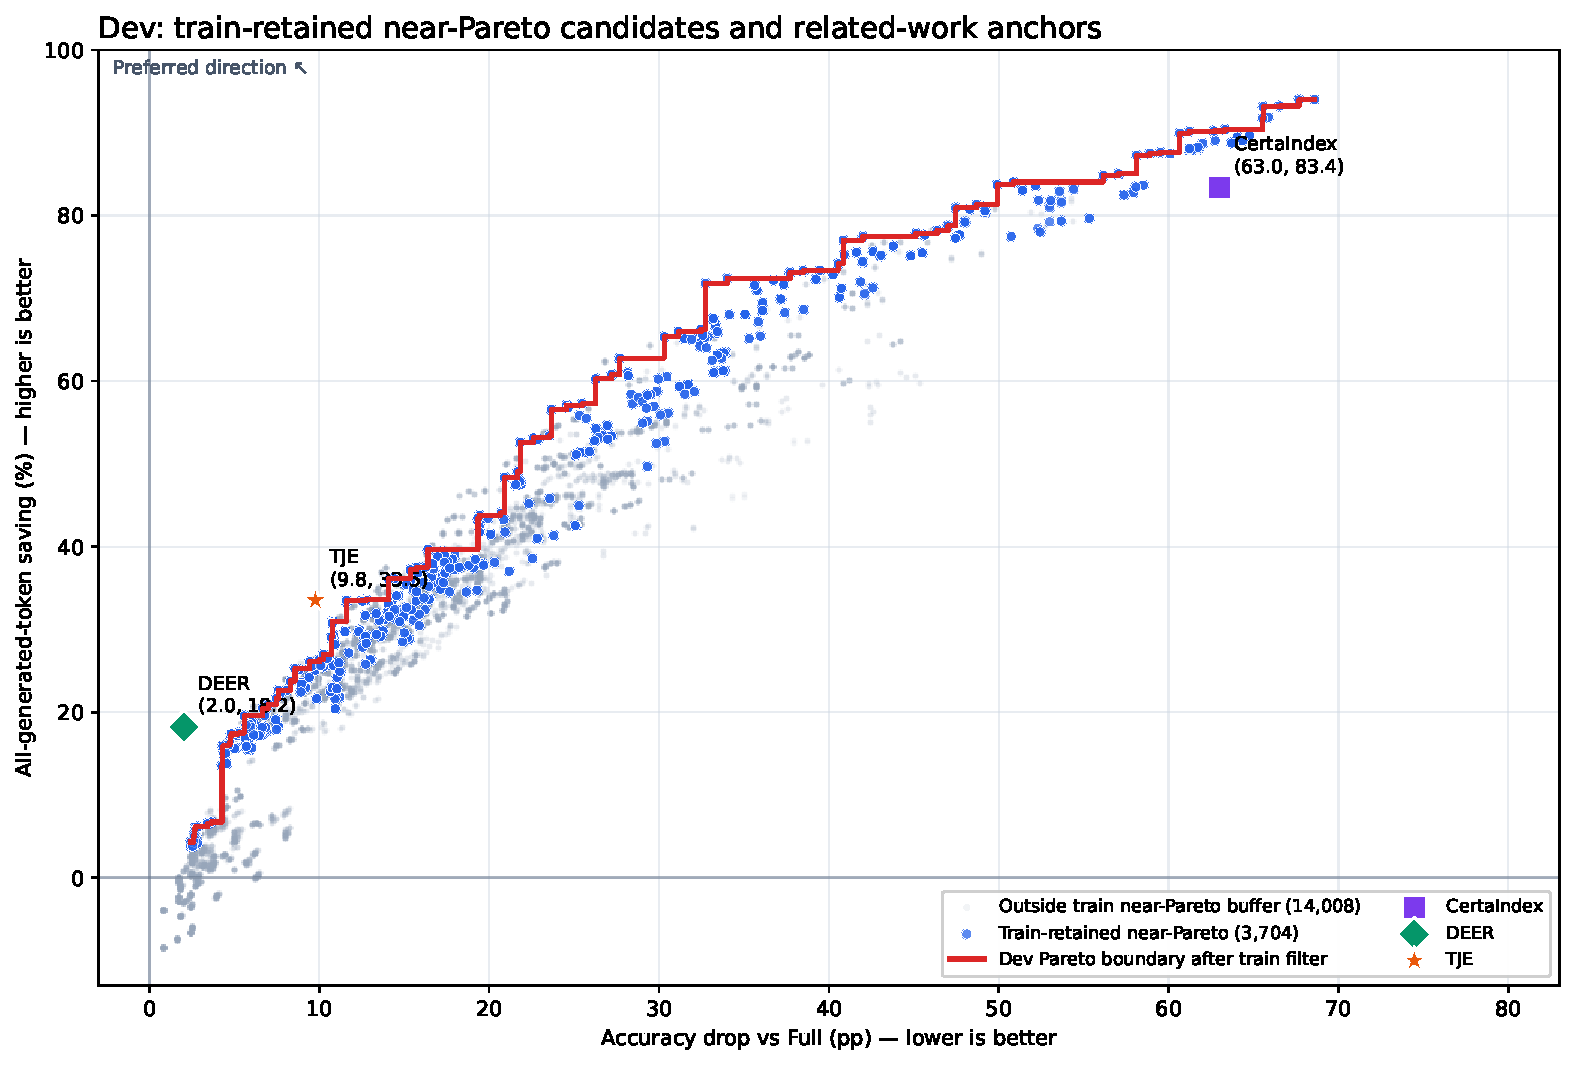
\includegraphics[width=\textwidth]{figures/governor_related_work_pareto_dev.pdf}
  \caption{\textbf{The safe-and-saving corner is empty.} Each grey point is one
  of the $17{,}712$ preregistered consensus rules on the development set; blue
  are the $3{,}704$ surviving a near-Pareto train filter, and the red step is the
  dev Pareto boundary. The top-left corner (small accuracy drop \emph{and} large
  token saving) contains no rule---the boundary only climbs as the drop grows.
  \textbf{CertaIndex} \citep{dynasor_certaindex}, the published consensus method,
  sits at the far right ($63\pp$ drop), the consensus family's collapse.
  \textbf{DEER} \citep{deer}, which reads a boundary-confidence signal
  \emph{outside} the swept space, occupies the low-drop corner
  ($2.0\pp$, $18\%$), above the consensus boundary at the same accuracy drop.
  The failure is a property of the consensus signal, not of early exit.}
  \label{fig:pareto}
\end{figure*}

\paragraph{Contribution.}
Our contribution is a rigorous, mechanism-backed demonstration that
\emph{intermediate answer-consensus is an unsafe early-exit signal for reasoning
LLMs}, established so that it cannot be waved away as an untuned heuristic. Three
components support this one claim:
\begin{itemize}
  \item \textbf{A preregistered, probe-independent test} (frozen trajectories,
  offline re-probing, a seven-dimensional $17{,}712$-rule schema, and selection
  gates fixed in advance) under which \emph{no} rule is both safe and
  token-saving---and which we release in full
  (Sections~\ref{sec:method}--\ref{sec:results}).
  \item \textbf{A mechanism} that explains \emph{why}: a directional
  ``continued-reasoning-corrects'' effect ($\approx\!35{:}1$) makes the accuracy
  cost of stopping intrinsic to the trajectory and independent of probe density,
  so the negative result generalizes beyond the searched schema
  (Section~\ref{sec:mechanism}).
  \item \textbf{Out-of-distribution and real-method confirmation}: the frontier
  reproduces on a held-out split and two unseen models, a published Certaindex
  reproduction collapses, and a non-consensus signal stays near full accuracy on
  the same trajectories---localizing the failure to consensus and indicating
  where a safe signal must come from (Sections~\ref{sec:results}--\ref{sec:mechanism}).
\end{itemize}
      % 1  Introduction (+ Figure 1, the climax)
\section{Related Work}
\label{sec:related}

\paragraph{Probe-based / consensus early exit.}
The methods we scrutinize periodically query a partial reasoning trajectory for
its current answer and halt on agreement. Dynasor / Certaindex
\citep{dynasor_certaindex} formalize this with a ``certainty index'' over recent
probe answers and use it to terminate early when serving reasoning programs, one
of several responses to the \emph{overthinking} of reasoning models
\citep{overthinking,deer}. We adopt the same probe mechanism (a short
boxed-answer suffix) and notion of probe agreement, and ask how far \emph{any}
rule in this family can be pushed before it becomes unsafe.

\paragraph{Early-stopping self-consistency and self-correction.}
Probe-based early exit is the online, \emph{single-trajectory} analogue of
early-stopping self-consistency
\citep{wang2023selfconsistency,aggarwal2023adaptive,li2024esc}: it votes across
snapshots of one in-progress trajectory rather than across finished samples. That
difference is the crux---snapshots of an unfinished trajectory are not
exchangeable draws from a stable answer distribution, because the trajectory is
still correcting itself. This intrinsic self-correction differs from the
prompted, post-hoc self-correction that \citet{huang2024selfcorrect} find
unreliable: we measure answer evolution \emph{within} one uninterrupted
trajectory, and find (Section~\ref{sec:results}) that a model's mid-trajectory
answer is far from final.

\paragraph{Alternative termination signals.}
Rather than probe agreement, a stop can read other signals: verifier- and
process-reward-guided decoding \citep{lightman2024verify,wang2024mathshepherd}
score partial reasoning, and adaptive-computation methods learn a halting signal
at the token or layer level \citep{graves2016act,schuster2022confident}. DEER
\citep{deer} stops on the model's confidence in a trial answer at reasoning
boundaries. We use DEER only as a \emph{positive control}
(Section~\ref{sec:mechanism}): run through the identical pipeline and acceptance
gates, it clears them where no consensus rule does, indicating that the failure
is specific to the probe-agreement signal rather than to early exit itself. We do
not claim this broader class of signals is categorically superior---our
experiments isolate one signal, not a taxonomy of methods.
Test-time scaling trades compute for accuracy via repeated sampling and search
\citep{snell2024scaling,brown2024monkeys}; early exit is its dual, spending less
without losing accuracy.

\paragraph{Preregistration.}
To keep an exhaustive rule search from silently overfitting to a favorable
operating point, we fix the rule schema, splits, and acceptance gates before
looking at held-out data \citep{preregistration_ml}. This preregistration
(Section~\ref{sec:method}) is what makes a \emph{negative} result interpretable.
      % 2  Related Work
\section{Method}
\label{sec:method}

To ask whether \emph{any}
probe-based rule can succeed, we need (i) an evaluation that a rule cannot game
by changing the reasoning it observes, and (ii) a selection procedure that
cannot silently overfit to a lucky operating point. We preregister both.

\subsection{Probe-independent, frozen trajectories}
For each problem we generate exactly \emph{one} main trajectory in a single
request (caps: $16$K tokens for \textsc{MATH}500 and AMC23, $32$K for AIME24)
and freeze it. All probing is then performed \emph{offline} against fixed text
prefixes of that frozen trajectory. Because probes never re-enter the decode,
changing a probe schedule---or a stopping rule---cannot change the underlying
reasoning; every rule is scored against the same trajectories. We build two
offline probe banks: a \emph{dense} bank that re-probes every $64$ tokens with
\simplek{} (a $32$-sample boxed-answer probe), and an \emph{adaptive} bank that
additionally fires event-triggered probes at entropy drops and at
conclusion/reflection/answer markers.

\subsection{Token accounting}
\label{sec:accounting}
For a rule that stops a problem at token position $s$ after consuming probe
output $p$, we charge total decode tokens $T=s+p$ and compare against the frozen
baseline $B$ (the full trajectory, capped at budget). \emph{Net} savings is
$(B-T)/B$ and \emph{gross} savings is $(B-s)/B$; their gap is the probe cost. The
accuracy drop compares the correctness of the committed answer at $s$ against that
of the frozen final answer (it is not an agreement rate between them). Two
quantities therefore move independently, and we track both: \emph{where} the rule
stops (setting the accuracy drop and the main-token saving $s$) and \emph{how much
it probes} to get there (adding $p$). Section~\ref{sec:mechanism} shows that only
the first is intrinsic.

\subsection{The consensus rule space $(W, s)$}
\label{sec:schema}
The consensus signal in the windowed family we study reduces to two
hyperparameters: a \textbf{window size} $W$ (how many of the most recent probes
to inspect) and a \textbf{share threshold} $s$ (what fraction of that window
must agree on a single answer before a stop is allowed). This pair spans the
family to a close approximation: $W{=}1$ is the ``latest-probe'' rule, $s{=}1.0$
is strict unanimity over the last $W$ probes (the CertaIndex-style stop), and an
entropy-over-the-window criterion closely tracks the same agreement and adds no
materially new operating point on our grid. We sweep $W\in\{1,3,5,8,12,16,24,30\}$ and
$s\in\{0.6,0.8,1.0\}$, deliberately including \emph{large} windows so a rule can
demand a long, stable agreement before committing.

Around this core we vary only the operational knobs that govern \emph{when} and
\emph{how} the signal is read: \textbf{probe schedule} (fixed interval
$\in\{64,128,256,512\}$ tokens, or event-triggered probing at
conclusion/entropy/reflection markers); \textbf{maturity} (a minimum-token floor
$\in\{0,512,1024,2048,4096\}$ before any stop is allowed); \textbf{validity} (an
answer-shape filter, rejecting empty/letter answers or only empties); and
\textbf{certainty} (optionally requiring the supporting probes to be flagged
certain). Enumerating this preregistered grid over a fixed-schedule and an
event-triggered family yields $3{,}520$ candidate consensus rules; formal
definitions are in Appendix~\ref{sec:appendix-schema}.

\paragraph{A better signal, swept identically.}
To test whether the failure is early exit \emph{itself} or the consensus
\emph{signal}, we sweep one non-consensus method through the same pipeline,
gates, and token accounting. \textbf{DEER} \citep{deer} stops on the model's own
confidence in a trial answer at a reasoning boundary; its only hyperparameter is
a confidence threshold, which we sweep over $14$ values. We use the stronger
\emph{trial-answer-submit} variant (commit the trial answer directly, no
separate readout) rather than the faithful readout reproduction---our aim here
is not to reproduce prior work but to ask whether \emph{any} rule can clear the
gates. Placing DEER and consensus on one frontier under identical accounting is
what makes the comparison a controlled test of the signal.

\subsection{Models, benchmarks, splits}
Development uses two models---\dsseven{} and \qweneight{}---on three benchmarks
(\textsc{MATH}500, AMC23, AIME24), each at seeds $42/43/44$: $18$
model$\times$benchmark$\times$seed environments. Problems are partitioned
\emph{by problem id} into $60/20/20$ train/dev/test splits
(\textsc{MATH}500 $300/100/100$, AMC23 $24/8/8$, AIME24 $18/6/6$), so no problem
leaks across splits. Confirmation reserves seeds $45/46/47$ plus two unseen
models---\mbox{DeepSeek-R1-Distill-Llama-8B} and \mbox{Distill-Qwen-32B}---all
evaluated on the \emph{test} split only. In one line: \emph{train} generates and
screens candidate rules in-sample, \emph{dev} is the sole selection target the
gates are read on, and \emph{test} (with the two unseen models) is read once for
confirmation after the rules and thresholds are frozen---never for tuning. Where
later sections say ``train+dev,'' they mean a rule was required to pass a gate
in-sample on train and is then measured on dev.

\subsection{Preregistered operating points and gates}
We fix three operating points and their acceptance gates \emph{before} looking
at held-out data (Table~\ref{tab:gates}). Each gate is applied in order:
first the \textbf{total accuracy drop} (macro-averaged over the $18$
environments) must stay under a cap; then the \textbf{total net token saving}
(macro-averaged) must clear a floor; and finally a \textbf{positive-saving
fraction} (psf, the fraction of environments with strictly positive net saving)
floor must be met. A rule is accepted at an operating point only if it satisfies
all three on train+dev. The saving floor is what distinguishes a genuinely
useful early exit from a rule that stays accurate only by almost never stopping.

\begin{table}[t]
  \centering\small
  \begin{tabular}{lccc}
    \toprule
    Operating point & Max total & Min total & psf \\
                    & acc.\ drop & saving    & floor \\
    \midrule
    conservative     & $1.0\pp$ & $10\%$ & $0.80$ \\
    balanced         & $2.0\pp$ & $20\%$ & $0.80$ \\
    token\_efficient & $3.5\pp$ & $30\%$ & $0.70$ \\
    \bottomrule
  \end{tabular}
  \caption{Preregistered acceptance gates. A rule must keep the macro-averaged
  accuracy drop under ``max total acc.\ drop,'' deliver at least ``min total
  saving'' net tokens, and post positive net saving on at least a psf fraction
  of environments. Gates are fixed in advance and \emph{not} relaxed post hoc.}
  \label{tab:gates}
\end{table}

\subsection{Metric resolution}
\label{sec:resolution}
The total accuracy drop is a macro-average over the $18$ environments (each
model$\times$benchmark$\times$seed weighted equally). We span two models, three
benchmarks, and three seeds and weight them equally so that selection rewards a
rule that is robust across benchmarks, models, and randomness, not one that
overfits a single setting. Pooling problems instead would let MATH500 ($100$ dev
problems per seed vs.\ $8$ for AMC23 and $6$ for AIME24) dominate the headline,
so a rule that wins only on MATH500 could pass; equal per-environment weight
forces a selected rule to hold on the harder competition sets too. Macro also
keeps any single problem from swinging the result---one AIME24 problem is
$16.7\pp$ of a $6$-problem split but only ${\sim}1/108$ of the macro drop---while
the three seeds damp the extra per-cell noise of the small sets. The gates are
read on the dev split (the selection target) with train reported alongside;
because \emph{no} consensus rule clears any gate by a wide margin
(Section~\ref{sec:results}), the finding does not rest on a single fragile cell.
Held-out confirmation on the test split and two unseen models provides the
complementary out-of-distribution check.

\subsection{Preregistration commitments}
Three commitments make the result interpretable. \textbf{(C1)} The test split
and both confirmation models are never read during rule selection.
\textbf{(C2)} All three operating points and their gates in
Table~\ref{tab:gates} are fixed before seeing held-out data and are not relaxed
afterwards; if no rule passes a gate, that is reported as the finding rather than
engineered away, and all three points are reported regardless of outcome.
\textbf{(C3)} The frozen rule set is fixed on train+dev and its hash recorded
before any test/confirmation evaluation. Section~\ref{sec:results} reports what
happened when we applied C2.
            % 3  Experimental Setup (frozen trajectories, accounting, splits)
\section{Analysis}
\label{sec:mechanism}

Section~\ref{sec:results} is an existence proof over $17{,}712$ rules, two seen
and two unseen models, and both splits. This section explains \emph{why} it holds
and why it generalizes beyond the exact rules we searched: the accuracy cost of
stopping on consensus is a directional property of the reasoning trajectory
itself, not of a threshold or of probe density.

\subsection{Stopping destroys more than it saves: a $35{:}1$ effect}
Consider only the stops where committing early \emph{changes} correctness relative
to the trajectory's own final answer, and count two outcomes: (final-correct,
stop-wrong)---a correct recovery destroyed---versus (final-wrong,
stop-correct)---a wrong answer luckily banked. Pure sampling noise predicts a
$\approx1{:}1$ ratio; a genuine ``continued reasoning corrects'' effect predicts
$\gg1$. On the frozen replay this ratio is $\mathbf{35{:}1}$ for the naive
consensus stopper ($1055$ destroyed vs.\ $30$ banked; $34.3{:}1$ and $35.9{:}1$ on
\dsseven{} and \qweneight{} separately) and $15$--$18{:}1$ for the more
conservative variants---all far above $1{:}1$. Stopping on consensus removes a
correct-in-the-end answer about $35$ times more often than it rescues a wrong one.
This is the recovery phenomenon of \S\ref{sec:exp-fc} ($65.5\%$, $76.3\%$), now at
the main $16$K/$32$K budgets and as a signed effect: the loss is real and
directional, not sampling variance.

\subsection{The accuracy tax is intrinsic to the trajectory}
Why is the ratio structural? For a rule stopping at token position $s$, the
accuracy drop depends only on $s$: committing at $s$ forgoes whatever correction
the trajectory would have made after it. It is a property of the reasoning, not of
the probe, so it survives \emph{any} probing scheme. This is what never reaches
zero in the sweep. The probe grid (intervals $64/128/256$ tokens) makes
essentially every stop position reachable and the observed floor is the minimum
over these schedules; a sparser schedule can only stop later or at a subset of
positions, never at a safer one the grid missed. Hence no threshold on the
consensus signal---in or beyond our schema---escapes the accuracy tax; the
searched space is a lower bound on the cost, not a lucky miss.

\subsection{Ruling out the ``it is just dense probing'' objection}
The natural rebuttal is that the negative result is an artifact of charging dense
re-probing. It is not, and separating two costs shows why. Besides the accuracy
tax, a rule pays a \emph{probe tax}: the probe output $p$ (Section~\ref{sec:accounting}).
Under dense re-probing a late-stopping rule pays $p$ over a long prefix, which
turns the \emph{net} savings of the safe (entropy) family negative even though its
\emph{gross} savings is positive (Table~\ref{tab:grossnet}). Unlike the accuracy
tax, the probe tax scales with probe density and is reducible (sparser or shorter
probes, KV-cache reuse). The two are separable: the \emph{savings} collapse is
partly a probe-tax artifact and is addressable, but the \emph{accuracy} floor is
probe-independent and is what makes the corner empty.

\begin{table}[t]
  \centering\small
  \begin{tabular}{lcc}
    \toprule
    Operating point & Gross saving & Net saving \\
                    & $(B-s)/B$    & $(B-s-p)/B$ \\
    \midrule
    Ours (target conservative)  & $+0.6\%$  & $-4.0\%$ \\
    Ours (target balanced)      & $+10.0\%$ & $+7.8\%$ \\
    Ours (target token\_efficient) & $+21.5\%$ & $+19.6\%$ \\
    \bottomrule
  \end{tabular}
  \caption{Gross vs.\ net savings; the gap is the probe tax. The
  target-conservative point's negative net saving is a probing-density artifact,
  not evidence that stopping wastes tokens---whereas the accuracy tax above it is
  intrinsic.}
  \label{tab:grossnet}
\end{table}

\subsection{It is the signal, not early exit}
The reproductions of \S\ref{sec:exp-prior} localize the cause. Every method that
stops on \emph{probe agreement}---the swept schema and CertaIndex alike---either
fails the safety bar or collapses outright; CertaIndex's $70\pp$ loss at $99.8\%$
stop rate is the accuracy tax paid in full. The lone method that stays near full
accuracy, DEER, does not read probe agreement at all: it stops on the model's own
confidence in a trial answer at a reasoning boundary, and in
Figure~\ref{fig:pareto} it sits \emph{above} the consensus Pareto boundary at the
same accuracy drop. This is direct evidence that the failure is a property of the
\emph{consensus signal}, not of early exit. (DEER's edge is model-dependent,
$+0.8\pp$ on \qweneight{} vs.\ $-4.8\pp$ on \dsseven{}, and these are
frozen-trajectory reproductions.)

\subsection{Implication: change the signal, not the threshold}
Much prior effort tunes consensus-based stops
\citep{dynasor_certaindex,aggarwal2023adaptive,li2024esc}; our frontier shows the
ceiling of that approach is low, and the mechanism above says no amount of tuning
raises it. The constructive implication is that a safe signal should be about
whether the \emph{trajectory itself} will still change, not about the agreement of
backward-looking probes. As a first step, we sketch in Appendix~\ref{sec:boundary}
an online controller built on DEER's boundary-confidence signal (fast-commit on
high confidence, else a verification branch) that recovers substantial savings at
near-neutral accuracy on dev; we stress it is exploratory (three seeds,
seed-sensitive, outside the preregistration) and report it only to show that
stepping outside the consensus-signal space escapes the accuracy tax we proved
unavoidable inside it. Verifier- and process-reward-based termination
\citep{lightman2024verify,wang2024mathshepherd} and learned halting
\citep{graves2016act,schuster2022confident} point the same way. Turning any of
these into a \emph{confirmed} method---with its own train/dev$\rightarrow$test
validation---is the natural next paper; our contribution is to establish
rigorously which signal not to build it on. Two caveats bound the claim: it
concerns \emph{consensus-based} rules within the searched schema and dense-probe
regime, and it does not say early exit is impossible---only that this signal
cannot make it safe.
         % 4  The Consensus--Termination Gap (discovery + mechanism)
\section{Experiments}
\label{sec:results}

Section~\ref{sec:mechanism} argues that probe agreement cannot make a stop safe
on its own, because the probes are not independent readings. The experiments here
establish that this is not a matter of tuning: we search the rule space
exhaustively and under commitment, and find nothing that escapes it.

We first confirm the phenomenon the paper turns on---intermediate consensus is
non-terminal (\S\ref{sec:exp-fc})---then report the preregistered sweep and its
central negative result: \emph{no} consensus rule is both safe and saving
(\S\ref{sec:exp-sweep}). We then show the failure is specific to the
\emph{signal}, not to early exit, by sweeping a non-consensus method (DEER)
through the identical pipeline and gates and finding that it \emph{does} clear
them (\S\ref{sec:exp-deer}); a released consensus stopper, CertaIndex (CoT),
shows the same failure at its default setting (\S\ref{sec:exp-prior}). Finally we confirm the frontier
out of distribution (\S\ref{sec:exp-heldout}).

\subsection{Non-Terminal Agreement}
\label{sec:exp-fc}
We log a dense probe stream for every \textsc{MATH}500 problem under \dsseven{}
at the main $16$K/$32$K budgets (all $500$ problems, three seeds; $1{,}500$
trajectories), never intervening---the probe is a separate forward pass that only
observes the main trajectory (full setup in Appendix~\ref{sec:appendix-fc})---and
read off four facts.

\textbf{(1) Final agreement is reliable; early agreement is not.} By the time a
trajectory finishes, agreement does track correctness: \emph{cumulative}
agreement across all probes is $97.8\%$ correct ($186$ trajectories reach it), and
even the final five-probe \emph{window} is $90.4\%$ correct ($1{,}205$). But an
online rule cannot wait for the end---it fires the \emph{first} time probes
agree, mid-trajectory, where the answer is far from settled (facts 2--4). The
operative question is not whether \emph{final} consensus is trustworthy, but
whether \emph{early} consensus is---and it is not.
\textbf{(2) Recovery is common.} Of the $1{,}148$ trajectories whose \emph{first}
probe is wrong, $89.1\%$ eventually flip to correct; of the $736$ that formed a
three-probe consensus \emph{different} from their final answer, $84.2\%$ ended up
correct.
\textbf{(3) Later consensus is worse.} Consensus formed before $512$ tokens is
$91.0\%$ correct, but consensus forming only after $2048$ tokens is $71.6\%$
correct---hard problems converge slowly \emph{and} to worse answers.
\textbf{(4) The cost lands at the stop.} A naive stop (first three consecutive
agreeing, certain, non-empty probes) fires on $1{,}477/1{,}500$ trajectories and
commits to answers correct only $50.5\%$ of the time, whereas letting those same
problems run to completion reaches $90.7\%$: a $40.2\pp$ loss.\footnote{A
simplified heuristic, \emph{not} the CertaIndex (CoT) rule (\S\ref{sec:exp-prior});
it fires early because the first stable, certain agreement is typically a
mid-trajectory placeholder. The swept rules below and the mechanism of
Section~\ref{sec:mechanism} quantify the same directional accuracy tax across the
full rule space.}

Figure~\ref{fig:consensus-pos} shows where this cost is concentrated. Expressing
the moment consensus first forms as a \emph{fraction} of each trajectory's own
length---which controls for problem difficulty---half of all consensuses form
within the first tenth of the trajectory, and there the answer they commit to is
correct only $27.5\%$ of the time against $85.2\%$ for the same problems run to
completion. The gap narrows as consensus forms later, but an online rule cannot
choose to wait: it fires when agreement first appears, which is precisely where
agreement is least informative.

A good stopping rule must therefore be much more than ``agreement.'' The rest of
this section asks whether the \emph{best possible} such rule, drawn from a large
preregistered space, can be both safe and economical.

\begin{figure}[t]
  \centering
  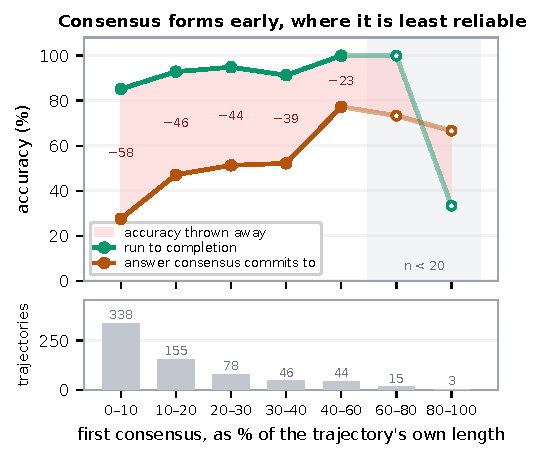
\includegraphics[width=\columnwidth]{figures/gen/fig_consensus_pos.pdf}
  \caption{\textbf{Consensus forms early, where it is least reliable.} For each
  dev-split trajectory we take the first window of three agreeing non-empty
  probes and ask two things: is that answer correct, and would the same problem
  have been correct if left to run? Position is a fraction of the trajectory's
  \emph{own} length, so $500$ tokens into a $600$-token trajectory counts as
  late and $500$ into a $16$K one does not. Consensus forms in $679$ of $684$
  trajectories, half within the first tenth; the shaded gap is the accuracy a
  stop at that moment throws away. Open markers mark bins with fewer than $20$
  trajectories; the final bin ($n{=}3$) should not be read.}
  \label{fig:consensus-pos}
\end{figure}

\subsection{Sweep Results}
\label{sec:exp-sweep}
We replay all $3{,}520$ consensus rules on the frozen trajectories and aggregate
to per-environment metrics---$126{,}720$ rows $=3{,}520$ rules $\times$ $18$
environments $\times$ $2$ splits (train, dev)---then, per rule, its total (macro)
accuracy drop and net token saving (accounting of Section~\ref{sec:accounting}).
Applying the preregistered gates yields the negative result that
Section~\ref{sec:mechanism} explains.

The outcome holds across environments: across all $126{,}720$ rule--environment
evaluations accuracy strictly \emph{falls} in $64.9\%$ and strictly \emph{rises}
in only $10.5\%$ (unchanged in $24.6\%$), for a mean drop of $13.0\pp$; over rules
the total dev drop has median $13.2\pp$ and a minimum of $0.81\pp$.
\textbf{Not one of the $3{,}520$ rules clears any gate.} The reason is the shape
of the trade-off, which Figure~\ref{fig:ws-heatmap} reads directly off the
sweep's own two axes: staying accurate and saving tokens are
in direct tension. Only $40$ rules keep the total drop at or below the
conservative $1.0\pp$ cap, and the most any of them saves is
$0.2\%$---far under the $10\%$ floor; conversely, the first rule to save $10\%$
already costs $2.66\pp$, saving $20\%$ costs $6.17\pp$, and saving $30\%$ costs
$11.8\pp$. Crucially, the sweep now includes \emph{large} windows (up to
$W{=}30$): these do buy low accuracy drop, but only by stopping so late that net
saving collapses to zero. No setting of the consensus signal escapes the
trade-off. Figure~\ref{fig:ws-heatmap} makes this a property of the whole
surface rather than of the frontier's edge: read cell by cell, the safest rule
available at each $(W,s)$ approaches the $1\pp$ cap only as the saving it buys
approaches zero, while every cell that saves substantially costs several points.
No cell clears the conservative gate.

\begin{figure*}[t]
  \centering
  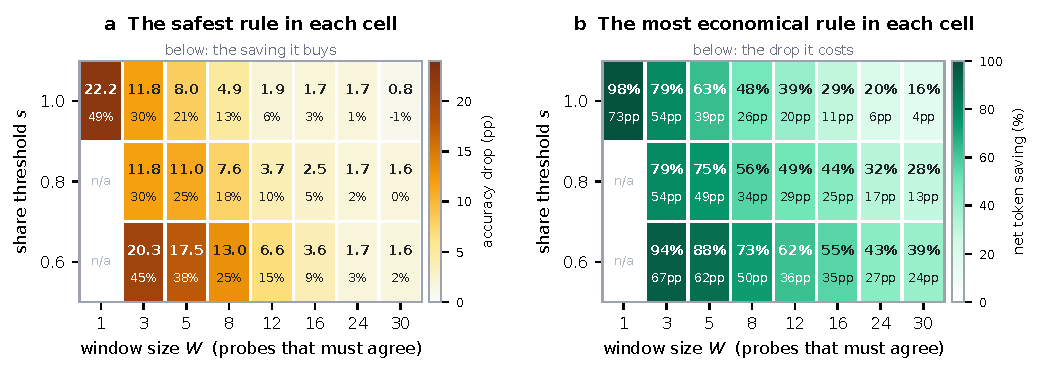
\includegraphics[width=\textwidth]{figures/gen/fig_ws_heatmap.pdf}
  \caption{\textbf{The safe-and-saving corner is empty across the entire rule
  space.} Dev split, macro-averaged over the $18$ environments. Each cell holds
  the $160$ rules that share its $(W,s)$ and differ only in the operational
  knobs, summarised by the two members a gate interrogates.
  \textbf{(a)} the cell's \emph{safest} rule: colour is its accuracy drop and
  the number beneath is the saving that rule buys. Larger windows and stricter
  thresholds do drive the drop towards the $1.0\pp$ cap---but the saving falls
  with it, reaching $-1\%$ at $W{=}30$, $s{=}1.0$.
  \textbf{(b)} the cell's \emph{most economical} rule: colour is its net saving
  and the number beneath is the drop it costs. Substantial saving is available
  everywhere, at $4$--$73\pp$. A cell would be outlined in green if any of its
  rules cleared the conservative gate (drop $\leq 1.0\pp$ \emph{and} saving
  $\geq 10\%$); none is.}
  \label{fig:ws-heatmap}
\end{figure*}

\subsection{A Non-Consensus Signal}
\label{sec:exp-deer}
The same gates are cleared, comfortably, by a rule that does \emph{not} read probe
agreement. Sweeping DEER's confidence threshold through the identical pipeline and
token accounting (Section~\ref{sec:schema}), its trial-answer-submit variant
passes all three operating points on dev: the conservative point loses only
$0.33\pp$ while saving $28.2\%$, the balanced point $1.03\pp$ at $29.6\%$, and the
token-efficient point $2.75\pp$ at $31.9\%$; at a stricter threshold it is
accuracy-neutral ($-0.06\pp$) while still saving $20.8\%$. Early exit is
therefore not impossible; the consensus \emph{signal} is what cannot make it
safe (Table~\ref{tab:main}).

\begin{table}[t]
  \centering\small
  \setlength{\tabcolsep}{4pt}
  \begin{tabular}{lccc}
    \toprule
    Method & Acc. & $\Delta$acc & Net \\
           &      & (macro)     & saving \\
    \midrule
    Full generation & $82.5\%$ & --- & $0\%$ \\
    \midrule
    Consensus (drop$\le1.0$)  & $81.6\%$ & $-0.9\pp$  & $+0.2\%$ \\
    Consensus (save$\ge10\%$) & $79.9\%$ & $-2.7\pp$  & $+10.7\%$ \\
    \midrule
    DEER (conservative)      & $82.5\%$ & $-0.33\pp$ & $+28.2\%$ \\
    DEER (balanced)          & $81.9\%$ & $-1.03\pp$ & $+29.6\%$ \\
    DEER (token\_eff.)       & $80.1\%$ & $-2.75\pp$ & $+31.9\%$ \\
    \bottomrule
  \end{tabular}
  \caption{Dev operating points (macro over $18$ environments). No consensus rule
  is simultaneously safe ($\le1.0\pp$) and saving ($\ge10\%$): capping the drop
  forces saving to near zero, and demanding saving forces a large drop. DEER,
  reading a non-consensus signal, clears all three gates on the same trajectories
  under the same accounting.}
  \label{tab:main}
\end{table}

\subsection{CertaIndex (CoT) at Its Default}
\label{sec:exp-prior}
The sweep covers rules we constructed; a released method lets us see where a
default setting lands. We reproduce two prior stoppers in a common harness---the
same frozen trajectories, the same token accounting.
\textbf{CertaIndex (CoT)} \citep{dynasor_certaindex} is the consensus stop for a
single chain of thought, reproduced from the released implementation at its
default \texttt{mid} setting: stop once three consecutive probes give the same
non-empty answer and none hedges. We use the authors' probe prompt and probe
schedule, so this is their rule as shipped, not a variant of ours.
\textbf{DEER} \citep{deer} here is the readout reproduction (the stronger
trial-answer-submit variant is what we swept in \S\ref{sec:exp-deer}).

Two scope notes. First, CertaIndex's multi-path setting is ordinary
self-consistency: it measures entropy over answers from \emph{independently
sampled} trajectories, and nothing here bears on it. What we reproduce is the
single-trajectory case, where the same statistic is read over repeated probes of
one chain. Second, Table~\ref{tab:baselines} reports these reproductions on our
frozen trajectories and benchmarks; it is not a re-run of either paper's
end-to-end system, and the original CoT results were reported on an easier
benchmark, where intermediate answers settle sooner.

\begin{table*}[t]
  \centering\small
  \begin{tabular}{llccccc}
    \toprule
    Method & Model & Accuracy & $\Delta$acc & Fair token saving & Stop rate & Signal \\
    \midrule
    Full generation & \qweneight{}   & $85.4\%$ & --- & $0\%$ & $0\%$ & --- \\
    Full generation & \dsseven{} & $79.8\%$ & --- & $0\%$ & $0\%$ & --- \\
    \midrule
    CertaIndex (CoT) & \qweneight{}   & $15.3\%$ & $-70.1\pp$ & $90.1\%$ & $99.8\%$ & consensus \\
    CertaIndex (CoT) & \dsseven{} & $23.9\%$ & $-55.9\pp$ & $76.7\%$ & $98.7\%$ & consensus \\
    \midrule
    DEER       & \qweneight{}   & $86.2\%$ & $\mathbf{+0.8\pp}$ & $16.3\%$ & $41.4\%$ & boundary conf. \\
    DEER       & \dsseven{} & $74.9\%$ & $-4.8\pp$  & $20.2\%$ & $56.1\%$ & boundary conf. \\
    \bottomrule
  \end{tabular}
  \caption{Prior early-stoppers reproduced on our frozen trajectories (dev, macro
  over three benchmarks; probe tokens charged). \textbf{CertaIndex (CoT)} stops on
  almost every problem and stops early, and loses $56$--$70\pp$ while saving
  $77$--$90\%$ of tokens---the pattern \S\ref{sec:exp-fc} describes, at a single
  shipped operating point. \textbf{DEER}, reading boundary confidence rather than
  probe agreement, stays near full accuracy ($+0.8\pp$ on \qweneight{}) while
  still saving tokens. These are reproductions on our benchmarks, not the original
  papers' end-to-end numbers; Section~\ref{sec:mechanism} interprets the
  contrast.}
  \label{tab:baselines}
\end{table*}

At a $99.8\%$ stop rate and $70\pp$ lost, CertaIndex (CoT) lands where the swept
consensus frontier says a rule at that stop rate must land. This is a property of
the signal, not a defect of the implementation: it is the same trade-off
\S\ref{sec:exp-sweep} maps across the whole rule space, seen at one shipped
operating point. The DEER readout, reading a non-consensus signal on the same
trajectories, stays near full accuracy; the stronger trial-answer-submit variant
we swept turns that into a gate-clearing frontier (\S\ref{sec:exp-deer}). That
only the non-consensus signal survives is what we analyze in
Section~\ref{sec:mechanism}.

\subsection{Generalization}
\label{sec:exp-heldout}
We read the test split once (commitment~C3). Because the development result is that
\emph{no} consensus rule clears any gate, there is nothing to confirm by
re-selection; we ask whether the \emph{frontier} reproduces, ranking rules on dev
and measuring on test.

\paragraph{Held-out test split.}
Each consensus rule's total drop on test tracks its dev value closely
($r=0.98$). The split-invariant claim is the empty \emph{joint} gate:
\textbf{no consensus rule clears the conservative gate on both splits}---$0$ on
dev, and the $444$ rules admissible on \emph{test alone} are exactly the
in-sample winners the held-out split exists to reject (all fail on dev). DEER, by
contrast, remains admissible across splits: $3$ of its thresholds clear the
conservative gate on \emph{both} dev and test (and $5$ clear balanced on both),
so the cross-signal contrast is not a dev artifact.

\paragraph{Unseen scale ($4\times$) and architecture.}
Both unseen models are evaluated on the test split at three seeds ($45/46/47$;
nine environments each), so their gates are as well resolved as development's. On
\mbox{Distill-Qwen-32B}, never used in development, the consensus frontier
reproduces ($r=0.97$ against dev drop); on the held-out architecture and family
\mbox{DeepSeek-R1-Distill-Llama-8B} it reproduces at $r=0.94$.\footnote{The
Llama-8B trajectories were re-collected after correcting a chat-template defect
(a missing model-specific beginning-of-sequence token that degraded its
generations); the corrected model scores $\sim\!88\%$ on \textsc{MATH}500.} The
\emph{conservative} gate stays empty on every model---dev, $32$B, and Llama all
admit $0$ rules (the best rule under a $1.0\pp$ drop saves $0.6\%$ on $32$B and
$9.3\%$ on Llama). At the looser gates a scale effect appears: on the $4\times$
larger $32$B a few consensus rules become admissible in-sample ($4$ at balanced,
$6$ at token-efficient), reflecting that a bigger model's intermediate answers
stabilize somewhat earlier---but these are not the dev-selected rules (dev admits
none), and on the same-scale Llama architecture the gates stay empty
($0/0/0$). Consensus thus yields no rule that is safe-and-saving where it is
selected, on any model. DEER, swept identically on these unseen models,
\textbf{clears the gates on both}: on \mbox{Qwen-32B} it is accuracy-neutral at
the conservative point ($-0.24\pp$ while saving $32.4\%$, $\tau{=}0.97$) and on
\mbox{Llama-8B} it loses $0.67\pp$ at $26.7\%$ ($\tau{=}0.99$), passing all three
gates. Consensus is unsafe, and DEER safe-and-saving, across all four axes we
vary---benchmark, seed, $4\times$ scale, and architecture/family.

Figure~\ref{fig:split-transfer} shows the selection pipeline end to end. The
$478$ consensus rules that clear the conservative gate in-sample on train are
tracked onto dev and test as a band; the three dev-selected DEER thresholds are
tracked individually. On dev---the split the gate is applied on---not one of the
$478$ is admissible, and the joint gate is empty, while all three DEER points
stay inside on every split. The dev and test splits are not equally demanding:
the same $478$ rules have a median drop of $4.5\pp$ on dev but $0.6\pp$ on test,
an asymmetry driven by the two smallest environments (AMC23 and AIME24 under
\qweneight{}, $8$ and $6$ problems), which carry the same weight as a
$100$-problem environment under macro-averaging. This is why the claim is stated
jointly rather than per split: $364$ of the $478$ are admissible on test, but
they are exactly the in-sample winners a held-out split exists to reject, and
none of them is selectable from dev.

Per-model and per-benchmark views of the same data, together with an
\emph{oracle} upper bound---a perfect probe-based stop committing the earliest
correct probe, which sits at a negative drop of $2$--$5\pp$ at $40$--$80\%$
saving, far in a corner neither method reaches---are given in
Appendix~\ref{sec:appendix-pareto}.

\begin{figure*}[t]
  \centering
  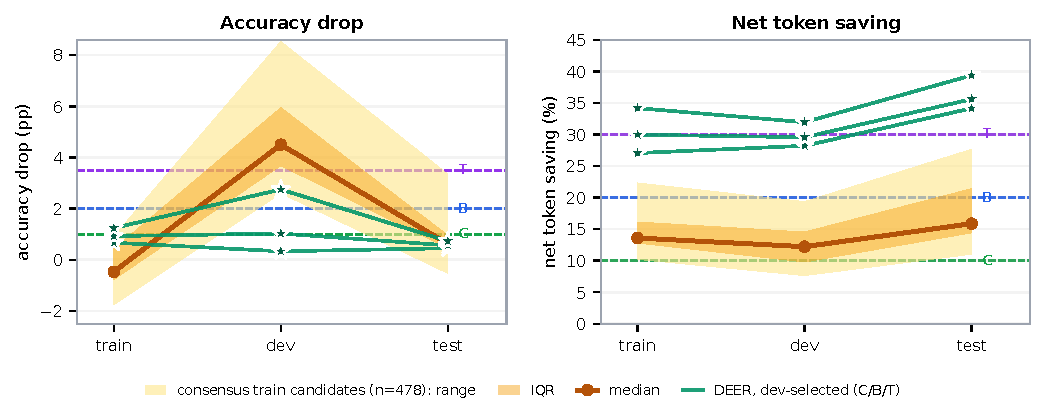
\includegraphics[width=\textwidth]{figures/gen/fig_split_transfer.pdf}
  \caption{\textbf{A rule must clear the gate on every split.} The $478$ amber
  rules are exactly those that clear the conservative gate \emph{in-sample on
  train}; drawing all $478$ would be unreadable, so we show their median,
  interquartile range and full range. Dashed lines mark all three preregistered
  gates (\textbf{C}onservative, \textbf{B}alanced, \textbf{T}oken-efficient);
  a rule must sit below them on the left and above them on the right. On dev,
  the split the gate is applied on, none of the $478$ does. Some recover on
  test, but a rule selected on dev is never among them: jointly, $0$ of $478$
  clear all three splits, against $3$ of $3$ for the DEER operating points
  selected on dev. Macro-averaged over $18$ environments per split; train and
  dev share seeds $42$--$44$ and differ only in problems, while test uses unseen
  problems and seeds $45$--$47$.}
  \label{fig:split-transfer}
\end{figure*}


           % 5  The Gap Cannot Be Tuned Away (sweep, DEER, wild, generalization)
\section{Conclusion}
\label{sec:conclusion}

Used on its own, self-consensus is not a safe early-exit signal: under a fixed
probing procedure agreement establishes that the current answer \emph{persists},
not that the reasoning has \emph{terminated}---a \emph{consensus--termination
gap}. What the probes agree on is often a placeholder forced from an unfinished
trajectory, so stopping destroys far more correct-in-the-end answers than it
rescues wrong ones, and more agreement only trades stopping opportunities
away. That asymmetry leaves the
safe-and-saving corner empty across $3{,}520$ preregistered rules, while a
boundary-confidence control swept through the same protocol clears every gate.
Agreement fails not because it is insufficiently strict, but because it
repeatedly measures the wrong object.
        % 6  Conclusion

\section*{Limitations}
\label{sec:limitations}

\paragraph{Development-set scope.}
The central result---no rule clears the conservative gate---is established on the
$18$ development environments (two models, three benchmarks, seeds $42/43/44$)
using the train and dev splits. Held-out confirmation on the test split and on
the two unseen models (Llama-8B, Qwen-32B) is \pending{not yet run}; the claim
is therefore currently a development-set finding. Because the effect sizes are
large (median frontier drop $20.1\pp$), we expect confirmation to reproduce the
direction, but the out-of-distribution magnitudes are not yet measured.

\paragraph{Small held-out sets on hard benchmarks.}
AIME24 and AMC23 are small; the dev split has only $6$ and $8$ problems per
seed, so a single problem is a large fraction. A worst-case per-model drop on
AIME24 can correspond to two or three problems, and is statistically noisy. We
mitigate by aggregating over seeds and reporting macro averages, but individual
per-benchmark cells should be read with this in mind.

\paragraph{Probe-tax dependence of the savings axis.}
Our net-savings numbers charge dense re-probing (every $64$ tokens, $32$-token
probes). A different probe schedule---sparser, shorter, or with KV-cache
reuse---would change the \emph{savings} axis and could move some rules from
negative to positive net savings. We separate gross from net savings
(Section~\ref{sec:mechanism}) precisely so that the probe-tax-dependent and
probe-tax-independent parts of the result are distinguishable; the accuracy-tax
result does not depend on the probe schedule.

\paragraph{Single probe suffix and rule space.}
We use one boxed-answer probe suffix (\simplek{}) and one preregistered rule
schema. Other probe wordings (e.g., the original Certaindex phrasing) and rule
dimensions outside this schema are not searched; a negative result is a
statement about the space searched, which we report explicitly ($17{,}712$
rules, four families, seven dimensions).

\paragraph{Domain.}
All benchmarks are competition mathematics with checkable final answers. Whether
false consensus and the accuracy tax transfer to open-ended reasoning, code, or
agentic tasks is out of scope here.
       % Limitations (unnumbered, ACL-required)

\bibliography{custom}

\appendix
\section{Rule Schema Details}
\label{sec:appendix-schema}

The seven-dimensional schema of Section~\ref{sec:method} enumerates to
$17{,}712$ candidate rules. Each rule fixes:
\begin{enumerate}
  \item \textbf{Probe schedule}: fixed interval $\in\{64,128,256\}$ tokens, or
  \texttt{adaptive\_event} with entropy-drop and marker triggers and a fallback
  interval.
  \item \textbf{Maturity}: \texttt{fixed\_tokens} (minimum tokens),
  \texttt{budget\_fraction} (minimum fraction of the decode budget), or
  \texttt{online\_instability} (a floor plus a same-answer stability check).
  \item \textbf{Evidence}: window share, latest persistence, or
  entropy-budget-fraction candidate selection.
  \item \textbf{Persistence}: minimum consistent accepts and minimum consensus
  span in tokens.
  \item \textbf{Certainty}: minimum fraction of supporting probes flagged
  certain.
  \item \textbf{Validity}: answer-shape filter (reject empty / single-letter
  answers to suppress the Type-E probe artifact of
  Appendix~\ref{sec:appendix-fc}).
  \item \textbf{History}: maximum answer switches within a window and minimum
  stable span since the last switch.
\end{enumerate}

\paragraph{Certainty.}
A probe is \emph{certain} when its boxed answer is emitted with high token-level
confidence: concretely, the mean probability of the answer tokens under the
probe forward pass exceeds a fixed threshold (the Certaindex certainty flag).
For the \simplek{} bank this is aggregated over the $32$ samples as the fraction
agreeing on the modal answer. Dimension~5 gates a stop on the fraction of the
supporting probes that are certain.

\paragraph{Entropy triggers.}
The \texttt{adaptive\_event} schedule fires an extra probe when the token-level
predictive entropy of the main decode drops by at least $\Delta H$ relative to a
trailing baseline (an ``the model just committed'' signal), and at
conclusion/reflection/answer marker tokens (e.g., ``therefore'', ``the answer
is''), subject to a minimum inter-probe gap and a fallback interval.

\section{Preregistration Text}
\label{sec:appendix-prereg}

The protocol version, split manifest hash, candidate-rule generation script, and
the three operating-point gates (Table~\ref{tab:gates}) were fixed before any
held-out evaluation. Commitments C1--C3 (Section~\ref{sec:method}) were recorded
with the protocol. When the conservative gate proved empty, we followed C2 and
report the empty gate as the finding rather than relaxing it; the
balanced/token\_efficient points are reported only as clearly-labeled post-hoc
analysis and would be re-preregistered if used for selection.

\section{Reproducibility}
\label{sec:appendix-repro}

Frozen trajectories, offline probe banks, the sweep archive
($637{,}632$ metric rows), and the aggregation scripts are released.
Table~\ref{tab:adaptive} was reproduced to the reported precision directly from
the released sweep archive. Grading uses a robust answer-equivalence check that
tries the raw and normalized reference forms and both string and
math-expression equality; per-problem correctness for the frozen baseline is
recomputed at replay time rather than trusted from collection.

\section{Family and Adaptive Frontiers}
\label{sec:appendix-tables}

Table~\ref{tab:frontier} gives each family's best attainable operating point on
dev (supporting Section~\ref{sec:results}): the simplest evidence signal
(\texttt{window\_share}) gives the best safe-with-positive-savings point, the
safest family (\texttt{entropy\_budget\_fraction}) cannot save, and the most
complex family (adaptive) is dominated by the simplest. Table~\ref{tab:adaptive}
isolates the adaptive frontier, showing it trades linearly into larger losses as
it grows aggressive.

\begin{table}[t]
  \centering\small
  \begin{tabular}{lcc}
    \toprule
    Rule family & Per-model & Net savings \\
                & drop (pp) & at that point \\
    \midrule
    \texttt{entropy\_budget\_fraction} & $1.85$ & negative ($q_{20}{\approx}{-}11\%$) \\
    \texttt{window\_share}             & $4.87$ & $\approx 0$ ($q_{20}{\approx}0.3\%$) \\
    \texttt{latest\_persistence}       & $8.20$ & $q_{20}{\approx}9.7\%$ \\
    \texttt{adaptive\_event\_probe}    & $9.70$ & $q_{20}{\approx}4.5\%$ \\
    \bottomrule
  \end{tabular}
  \caption{Best operating point per rule family on dev. For
  \texttt{entropy\_budget\_fraction} we show its \emph{absolute} minimum drop
  (which has no positive-savings point); for the other three families we show the
  minimum worst-case per-model drop \emph{among positive-savings points}. The
  safest family cannot save; the most complex family (adaptive) is dominated by
  the simplest (window share).}
  \label{tab:frontier}
\end{table}

\begin{table}[t]
  \centering\small
  \begin{tabular}{lcccc}
    \toprule
    Adaptive point & Trigger & Mean & $q_{20}$ & Macro \\
                   &         & save & save     & $\Delta$acc \\
    \midrule
    conservative & entropy drop & $14.2\%$ & $4.5\%$  & $-5.88\pp$  \\
    moderate     & conclusion   & $25.9\%$ & $20.0\%$ & $-9.11\pp$  \\
    aggressive   & conclusion   & $37.3\%$ & $27.1\%$ & $-15.03\pp$ \\
    \bottomrule
  \end{tabular}
  \caption{The \texttt{adaptive\_event\_probe} frontier on dev. Worst
  per-model/per-benchmark drops for the three points are
  $-9.70/-10.42$, $-13.65/-12.50$, and $-19.28/-18.75\pp$ respectively.
  Reproduced exactly from the released sweep archive.}
  \label{tab:adaptive}
\end{table}
                 % A  Rule schema, preregistration, reproducibility, tables
\section{False Consensus: Full Analysis}
\label{sec:appendix-fc}

Section~\ref{sec:related} summarizes the four facts this appendix establishes in
full, in an intervention-free setting: that intermediate probe consensus is not a
reliable stopping signal.

\subsection{Setup}
\label{sec:fc-setup}
We run \dsseven{} (vLLM, one A100-80G) on all $500$ \textsc{MATH}500 problems
\citep{lightman2024verify,hendrycks2021math} with a decode budget of $3072$
tokens, temperature $0.6$, top-$p$ $0.95$, and seed $42$. Every $128$ generated
tokens (at most $24$ probes per problem) we append the boxed-answer probe
suffix and read off the model's current answer. The probe is a separate forward
pass: the controller only \emph{observes}, never halting or altering the main
trajectory. This yields, per problem, the full answer trajectory a stopping rule
would have access to. This exploratory study uses a deliberately tight $3072$
budget so that many trajectories are truncated and the ``continue vs.\ stop''
contrast is visible within one A100; the preregistered sweep
(Section~\ref{sec:method}) re-examines the phenomenon at the $16$K/$32$K budgets
used for the main results, and we report the recovery statistics there as well.

\subsection{Agreement is not correctness}
We compare two notions of probe agreement.
\emph{Cumulative} agreement (all non-empty probes so far concur) is nearly
trustworthy: on the $87$ problems that reach unanimous cumulative agreement,
$98.9\%$ are correct, with a single whole-trajectory false consensus. But
cumulative agreement is not what an online stopping rule sees. The operative
signal is \emph{window} agreement---the last five probes concurring---and it is
markedly less reliable: of the $338$ problems reaching a unanimous last-five
window, only $93.5\%$ are correct, giving a $6.5\%$ ($22/338$) false-consensus
rate. Perfect \emph{global} consensus is almost safe; the \emph{local} consensus
a controller must act on is not.

\subsection{The cost lands at the stopping decision}
We simulate a \emph{naive consecutive-agreement} stop: halt at the first point
where three consecutive probes agree, are non-empty, and are \emph{certain}
(the model emits the boxed answer with high token-level confidence; formal
definition in Appendix~\ref{sec:appendix-schema}). This is a simplified
heuristic, \emph{not} the Certaindex algorithm, which we reproduce faithfully in
\S\ref{sec:exp-prior}. It fires on $416/500$ problems. The committed
answers are correct only $69.2\%$ of the time, whereas letting those same
problems run to completion (within the $3072$ budget) reaches $85.6\%$---a
\textbf{$16.4\pp$ accuracy loss} in exchange for an average saving of $1321$
tokens, with $128$ problems stopped on an outright wrong answer.

\subsection{Recovery is common, and early stopping kills it}
The loss is driven by \emph{recovery}: continued reasoning overturns the
intermediate answer far more often than intuition suggests. Of the $145$
problems that at some point formed a three-probe consensus \emph{different} from
their final answer, $95$ ($65.5\%$) ended up correct; and of the $375$ problems
whose \emph{first} probe was wrong, $76.3\%$ eventually flipped to correct.
Neither ``first impression'' nor ``local consensus'' is close to terminal.

Counterintuitively, \emph{later} consensus is \emph{less} trustworthy:
consensus formed before $512$ tokens is $87.4\%$ correct, but consensus that
only forms after $2048$ tokens is $58.1\%$ correct. Hard problems both converge
slowly and converge to worse answers---exactly the problems on which an
aggressive stopping rule does most damage.

\subsection{Miscalibration}
Window share is a poorly calibrated confidence estimate. Its calibration
error---the gap between share and empirical accuracy, averaged over share bins
(CCE)---is $0.080$ (versus $0.149$ for cumulative share), but the error is
concentrated where a rule would act: at window share $0.8$ the empirical
accuracy is only $47.2\%$ ($n{=}36$). A threshold tuned to ``looks nearly
unanimous'' is operating precisely in the band where the signal is least
reliable.

\subsection{An error taxonomy}
Hand-inspecting stopped-but-wrong cases ($28$ cases from the first $100$
problems; AI-assisted labeling, treated as preliminary) yields \emph{four}
non-empty types out of five categories.
By count: \textbf{(A)} numeric collapse---stable convergence to a wrong
number---$14/28$; \textbf{(D)} derivation gaps---dropped roots/cases, unverified
solutions---$7/28$; \textbf{(E)} format/option hallucination---a
non-multiple-choice problem stably emitting a letter such as ``B''---$6/28$,
which is an artifact of the probe mechanism itself rather than a model belief;
and \textbf{(B)} expression collapse---$1/28$. Type~\textbf{(C)} (sign errors)
did not occur in this sample. Type~E is itself a methodological finding: roughly
one in five ``false consensuses'' is a probe formatting artifact, implying that
any deployed rule should filter answer \emph{shape}.

\paragraph{Takeaway.}
These observations---local consensus unreliable, recovery common, late
consensus worse, confidence miscalibrated---suggest that a good stopping rule
must be much more than ``agreement.'' The rest of the paper asks whether the
\emph{best possible} such rule, drawn from a large preregistered space, can be
both safe and economical. In the searched space, it cannot.
         % B  Self-consensus: full analysis

\end{document}
